\documentclass{article}
\usepackage[latin1]{inputenc}
\usepackage[T1]{fontenc}
\usepackage{graphicx}
\usepackage{subfigure}
\usepackage{cite}
\usepackage[obeyspaces]{url}
\usepackage{tikz}
\usepackage{geometry}
\geometry{paperheight=15.5cm, paperwidth=12cm, margin={2mm,2mm}}
\usetikzlibrary{calc,positioning,shapes.geometric}
\begin{document}
\newcommand*\circled[1]{\tikz[baseline=(char.base)]{
		\node[shape=circle,fill=white,draw,minimum size = 0.5cm, inner sep=2pt] (char) {#1};}}
  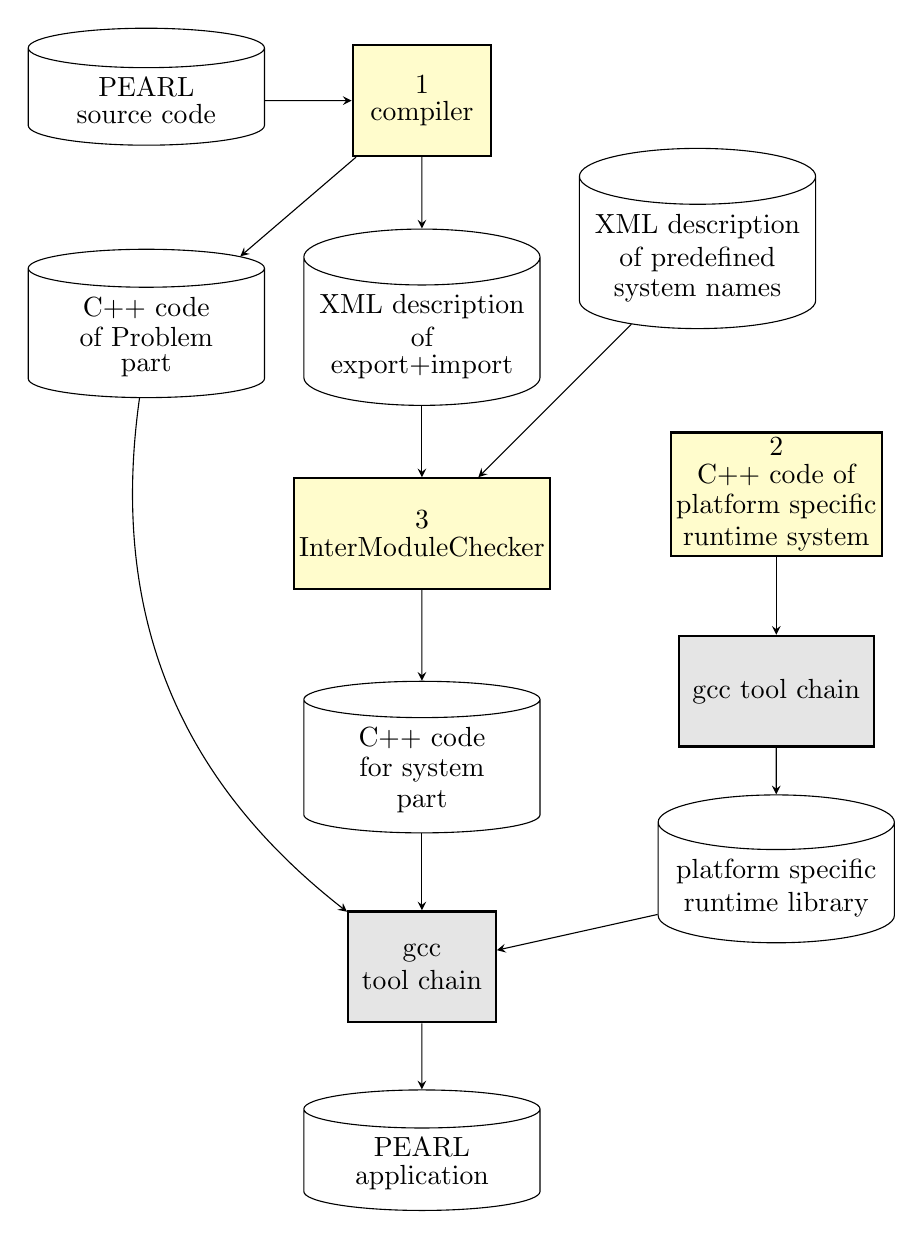
\begin{tikzpicture}[
    >=stealth,
    node distance=3.5cm,
    file/.style={
      cylinder,
      cylinder uses custom fill,
      %cylinder body fill=yellow!50,
      %cylinder end fill=yellow!50,
      shape border rotate=90,
      minimum width=3cm,
      aspect=0.25,
      draw
    },
    fileold/.style={
          cylinder,
          cylinder uses custom fill,
          cylinder body fill=gray!20,
          cylinder end fill=gray!20,
          shape border rotate=90,
          minimum width=3cm,
          aspect=0.25,
          draw
        },
    block/.style = { rectangle,
    				draw=black,
    				 thick, 
                    %fill=blue!20,
                    text centered, minimum width=5em,
                    %rounded corners,
                    inner sep = 2pt,
                    minimum height=4em },
    blockold/.style = { rectangle,
       				draw=black,
       				 thick, 
                       fill=gray!20,
                       text centered, minimum width=5em,
                       %rounded corners,
                       inner sep = 0.5em,
                       minimum height=4em }                         
  ]
    \node[file] (prl) at (0,10) {\shortstack{PEARL\\source code}};
    \node[block, fill=yellow!20, right of=prl] (sprachumsetzer)  {\shortstack{\circled{1}\\ compiler}};
    \node[file,below of=prl,yshift=0.5cm] (problemcc) {\shortstack{C++ code\\of Problem\\part}};
    \node[file,below of=sprachumsetzer,yshift=0.5cm] (modulxml) {\shortstack{XML description
                                                            \\of \\
                                                             export+import}};
    \draw[->] (prl) -- (sprachumsetzer);
    \draw[->] (sprachumsetzer) -- (problemcc);
    \draw[->] (sprachumsetzer) -- (modulxml);

    \node[file, yshift=1cm,right of=modulxml] (hardwarexml) {\shortstack{XML description \\of predefined\\system names}};
    \node[block, fill=yellow!20,below of=modulxml,yshift=1cm] (imc) {\shortstack{\circled{3}\\ InterModuleChecker}};

    \draw [->] (modulxml) --  (imc);
    \draw [->] (hardwarexml) -- (imc);
    
    \node[file, below of=imc,yshift=0.5cm] (systemcc) {\shortstack{C++ code\\ for system  \\part}};
    \node[blockold, below of=systemcc,yshift=1cm] (gcc)
    {{\shortstack{gcc\\tool chain}}};


   \node[file, right of=gcc, xshift=1cm,yshift=1cm] (runtimelib)
{\shortstack{platform specific \\ runtime library}};
   \node[blockold, above of=runtimelib, yshift=-1cm] (gcc1){gcc tool chain};
   \node[block, above of=gcc1,fill=yellow!20,yshift=-1cm] (runtimepackage)
{\shortstack{\circled{2} \\C++ code of \\ platform specific \\ runtime system}};
    \draw[->] (runtimepackage) -- (gcc1);
    \draw[->] (gcc1) -- (runtimelib);

    \draw[->] (imc) -- (systemcc);
    \draw[->] (systemcc) -- (gcc);
    \draw[->] (runtimelib) -- (gcc);
    \draw[->] (problemcc) to[bend right] (gcc);
    
    \node[file, below of=gcc,yshift=1cm] (pearlapp) {\shortstack{PEARL\\application}};
    \draw[->] (gcc) -- (pearlapp);
  \end{tikzpicture}
\end{document}